% !TEX root = main.tex

Molecular Dynamics campaigns are significant consumer of computing cycles and
produce immense amounts of data, especially during simulation stages. Simulation
workflows execute up to $10^5$ $\mu sec$ MD simulations of a $O(100k)$ atoms
physical system, producing from $O(10)$ to $O(1000)$ GBs of
data~\cite{cheatham2015impact}. Increasingly, there is a need for analyses to be
integrated with simulations to drive the next stages of the workflow execution
at runtime~\cite{balasubramanian2016extasy}. Analyses can benefit from
task-level parallelism as they can be partitioned into independent units of
work.

Task-parallel applications involve partitioning a workflow into a set of
self-contained units of work. Based on the application, these tasks can be
independent, have no inter-task communication, or coupled with varying degrees
of data dependencies. Data-intensive applications exploit task parallelism for
data-parallel operations (e.g., \texttt{map}), but also require coupling, for
computing aggregates (\texttt{reduce}). Typically, a reduce operation includes
shuffling intermediate data from a set of nodes to node(s) where the reduce
executes.

Data analytics workflow engines exploit task-parallelism by partitioning the
data and generating stages of independent tasks. These stages then implement
data dependencies by shuffling, aggregating or coupling intermediate results.
The MapReduce~\cite{dean2004mapreduce} abstraction, along with its
implementations, popularized this method of processing.

Spark~\cite{zaharia2010spark} and Dask~\cite{rocklin2015dask} are two MapReduce
frameworks. Both provide abstractions which reason about data and are optimized
for parallel processing of large data volumes, interactive analytics and machine
learning. Their runtime engines can automatically partition data, generate
parallel tasks, and execute them on a cluster. In addition, Spark offers
in-memory capabilities allowing data caching data, making it suited for
interactive analytics and iterative machine learning algorithms. Dask also
provides a MapReduce API (Dask Bags). Furthermore, Dask's API is more versatile,
allowing custom workflows and parallel vector/matrix computations.

As task-parallel frameworks offer different abstractions and capabilities,
executing data analysis workflows in an efficient and scalable manner remains a
challenge. As data analysis applications can have different characteristics
(e.g., embarrassingly parallel or MapReduce), alternative abstractions and
capabilities may offer varying performance and efficiency. As a result, there is
a need to understand which framework is more suitable for performing a specific
type of analysis.

In this chapter, we investigate three task-parallel frameworks and their
suitability for implementing MD trajectory analysis algorithms. In addition to
Spark and Dask, we investigate RADICAL-Pilot (RP)~\cite{merzky2019using}. We utilize
MPI4py~\cite{dalcin2005mpi} to provide MPI equivalent implementations of the
algorithms. The task-parallel implementations performance and scalability
compared to MPI is the basis of our analysis. MD trajectories are time series of
atoms/particles positions and velocities, which are analyzed using different
statistical methods to infer certain properties, e.g., the relationship between
distinct trajectories, snapshots of a trajectory etc.

The chapter is organized as follows: ~\S\ref{sec:tp_related_work} discusses
several approaches to support scalable MD trajectory data analytics.
~\S\ref{sec:md_use_cases} describes the MD analysis algorithms investigated
and reviews different MD analysis frameworks with respect to their ability to
support scalable analytics of large volumes of MD trajectories.
~\S\ref{sec:frameworks} describes RP, Spark and  Dask, the three
frameworks used for our performance comparison and evaluation.
~\S\ref{sec:impl_exp} provides a description of the implementation of the
MD algorithms on top of those three frameworks, as well as a performance
evaluation and a discussion of our findings. In
~\S\ref{sec:task_sel_model}, we provide a conceptual analysis that allows
application developers to select a framework according to their requirements.
Finally, ~\S\ref{sec:tp_concl} closes this chapter with our conclusions.

%\mtnote{In Chapter 2 you use \S for section, here you use "s|Section \#"}

\section{Related Work}
\label{sec:tp_related_work}

Until recently, MD analysis algorithms were executed serially and
parallelization was not straightforward. During the last years, several
frameworks emerged providing parallel algorithms for analyzing MD trajectories.
Some of those frameworks are CPPTraj~\cite{roe2013ptraj,roe2018parallelization},
HiMach~\cite{tiankai2008scalable}, PMDA~\cite{fan2019pmda}, Pteros
2.0~\cite{yesylevskyy2015pteros} and nMoldyn-3~\cite{hinsen2012nmoldyn}.

Several techniques are used for parallelizing MD analysis algorithms.
CPPTraj~\cite{roe2018parallelization} utilizes MPI and OpenMP to execute
large-scale analysis on HPC. OpenMP is also utilized by
Pteros~\cite{yesylevskyy2015pteros} to parallelize the compute intensive parts
of the analysis. HiMach~~\cite{tiankai2008scalable} extends Google's MapReduce
and defines Map and Reduce methods. nMoldyn-3~\cite{hinsen2012nmoldyn}
parallelizes the execution through a Master/Worker architecture. The master
defines analysis tasks which are then executed by a set of worker processes.

%HiMach~\cite{tiankai2008scalable} was developed by D. E. Shaw Research group to
%provide a parallel analysis framework for MD simulations, and extends Google's
%MapReduce. HiMach API defines trajectories, does per frame data acquisition
%(Map) and cross-frame analysis (Reduce). HiMach's runtime is responsible to
%parallelize and distribute Map and Reduce phases to resources. Data transfers
%are done through a communication protocol created specifically for HiMach.

%Pteros-2.0~\cite{yesylevskyy2015pteros} is a open-source library that is used
%for modeling and analyzing MD trajectories, providing a plugin for each
%supported algorithm. The execution is done by a user defined driver
%application, which setups trajectory  I/O and frame dispatch for analysis. It
%offers a C++ and Python API. Pteros 2.0 parallelizes computational intensive
%algorithms via OpenMP and Multithreading. As a result, it is bounded to execute
%on a single node, making any analysis execution highly dependent on memory
%size. Through RP, Spark and Dask, we avoided recompiling every time
%there is a change to the underlying resource, ensuring the application's
%execution.

%MDTraj~\cite{mcgibbon2015mdtraj} is a Python package for analyzing MD
%trajectories. It links MD data and Python statistical and visualization
%software. MDTraj proposes parallelizing the execution by using the parallel
%package of IPython as a wrapper along with an out-of-core trajectory reading
%method. Our approach allows data parallelization on any level of the execution,
%not only in data read.

%nMoldyn-3~\cite{hinsen2012nmoldyn} parallelizes the execution through a Master
%Worker architecture. The master defines analysis tasks, submits them to a task
%manager, which then are executed by the worker process. In addition, it
%provides adaptability, allowing on-the-fly addition of resources, and execution
%fault tolerance when worker processes disconnect.

A common denominator of most approaches is that they do not use general purpose
frameworks for parallelizing the execution. Although they are optimized to get
as much performance as possible from the environments they are developed for,
their portability is limited. For example, CPPTraj~\cite{roe2018parallelization}
and Pteros~\cite{yesylevskyy2015pteros} are highly dependent on the low level
libraries of the resource they use, while HiMach~\cite{tiankai2008scalable} is
build specifically for the Antons Supercomputer.

In contrast, our analysis focuses on frameworks that offer more general
purpose approaches to the parallelizing MD analysis algorithms.
%Specifically, PMDA utilizes Dask to parallelize MD Trajectory analysis.
These frameworks provide higher-level abstractions that facilitate the
integration with other data analysis methods. In addition, resource acquisition
and management is done transparently.

\section{Molecular Dynamics (MD) Data Analysis}
\label{sec:md_use_cases}

Root Mean Square Deviation (RMSD), Pairwise Distances (PD), and
Sub-setting~\cite{mura2014biomolecules} are algorithms commonly used to analyze
MD trajectories. Path Similarity Analysis (PSA)~\cite{seyler2015path} and
Leaflet Identification~\cite{michaud2011mdanalysis} are two more advanced
algorithms. All these methods read and process a physical system generated via
multiple simulations, reducing data to either a single number or a matrix. RMSD
identifies the deviation of atom positions among frames, while PD and PSA
calculate distances between atoms or trajectories based on different metrics.
Sub-setting methods are used instead to isolate parts of interest of a MD
simulation, and Leaflet Identification provides information about groups of
lipids by identifying the lipid leaflets in a lipid bilayer.

We discuss two of those methods---a PSA algorithm that uses the Hausdorff
distance and a Leaflet identification algorithm---implementated in
MDAnalysis~\cite{michaud2011mdanalysis,gowers2016mdanalysis}.
%Section~\ref{ssec:mda} discusses the reasons for selecting these two algorithms
%in more detail.
%In addition, we implemented the PSA algorithm using CPPTraj~\cite{roe2013ptraj}.
%Furthermore, we explore the applications' Ogres Facets and Views~\cite{fox2014towards}, which provide a more systematic characterization.
%Big Data Ogres~\cite{fox2014towards} are organized into four classes, called \emph{views}.
%The possible features of a view are called \emph{facets}.
%A combination of facets from all views defines an Ogre.
%The Views are:
%\begin{inparaenum}[1)]
%    \item execution - describes aspects, such as I/O, memory, compute ratios, whether computations are iterative, and the 5 V's of Big Data (Volume, Velocity, Value, Variety and Veracity),
%    \item data source \& style - discusses input data collection, storage and access,
%    \item processing - describes algorithms and kernels used for computation, and
%    \item problem architecture - describes the application architecture.
%\end{inparaenum}
%\subsection{Applications and Algorithms}
%\label{ssec:mda}
MDAnalysis is a Python library~\cite{michaud2011mdanalysis,gowers2016mdanalysis}
that provides a comprehensive environment for filtering, transforming and
analyzing MD trajectories. MDAnalysis provides
a common object-oriented API to trajectory data and leverages existing libraries
of the scientific Python software stack, such as NumPy~\cite{numpy} and
Scipy~\cite{scipy}.

\subsubsection*{Path Similarity Analysis (PSA): Hausdorff Distance}

Path Similarity Analysis (PSA)~\cite{seyler2015path} quantifies the
similarity between trajectories, considering their full atomic detail. The
basic idea is to compute pair-wise distances (e.g., using the Hausdorff
metric~\cite{huttenlocher1993comparing}) between members of an ensemble of
trajectories, and cluster the trajectories based on their distance matrix. Each
trajectory is represented as a two dimensional array: The first dimension
corresponds to time frames of the trajectory; the second to the $N$ atom
positions in a 3-dimensional space. Algorithm~\ref{alg:hausdorff} describes
PSA with the Hausdorff metric over multiple trajectories. We apply a 2-dimensional
data partitioning over the output matrix to parallelize, shown in
algorithm~\ref{alg:partition}.

\begin{algorithm}[t]
    \scriptsize
    \caption{Path Similarity Algorithm: Hausdorff Distance}
    \label{alg:hausdorff}
    \begin{algorithmic}[1]
        \Procedure{HausdorffDistance}{$T_1$,$T_2$}\Comment{$T_1$ and $T_2$ are a set of
            3D points}
        \State \texttt{List $D_1$,$D_2$}
        \For{$\forall frame_1$ in $T_1$}
        \For{$\forall frame_2$ in $T_2$}
        \State \texttt{Append in $D_1$ $d_{RMS}$($frame_1$, $frame_2$)}
        \EndFor
        \State \texttt{$D_{t_1}$ append $min(D_1)$}
        \EndFor
        \For{$\forall frame_2$ in $T_2$}
        \For{$\forall frame_1$ in $T_1$}
        \State \texttt{Append in $D_2$ $d_{RMS}$($frame_2$, $frame_1$)}
        \EndFor
        \State\texttt{$D_{t_2}$ append $min(D_2)$}
        \EndFor
        \State \textbf{return} $max\Big(max(D_{t_1}),max(D_{t_2})\Big)$
        \EndProcedure
        \\
        \Procedure{PSA}{$Traj$}\Comment{$Traj$ is a set of trajectories}
        \For{$\forall T_1$ in $Traj$}
        \For{$\forall T_2$ in $Traj$}
        \State \texttt{ $D_{( T_1,T_2 )}$=HausdorffDistance$\Big( T_1,T_2 \Big)$}
        \EndFor
        \EndFor
        \State \Return $D$
        \EndProcedure
    \end{algorithmic}
\end{algorithm}


\begin{algorithm}[t]
    \scriptsize
    \caption{Two Dimensional Partitioning}
    \label{alg:partition}
    \begin{algorithmic}[1]
        \State Initially, there are $N^2$ distances, where $N$ is the number of trajectories.
        Each distance defines a computation task.
        \State Map the initial set to a smaller set with $k=N/n_1$ elements, where $n_1$ is a divisor of $N$, by grouping $n_1$ by $n_1$ elements together.
        \State Execute over the new set with $k^2$ tasks.
        Each task is the comparisons between $n_1$ and $n_1$  elements of the initial set.
        They are executed serially.
    \end{algorithmic}
\end{algorithm}

The algorithm is embarrassingly parallel, has complexity $O(n^2)$ and its input
data volume is medium to large while the output is small.
Embarrassingly parallel algorithms are good candidates for task parallelization.
Each task analyzes a partition of the dataset. Given
enough resources, tasks can execute concurrently as a bag of tasks, using a task
management API or a map-only application in a MapReduce-style API. Spark, Dask
and RP support the execution of bag of tasks, with RP and
Dask offering specific abstractions (as discussed in~\S\ref{sec:frameworks}).

\subsubsection*{Leaflet Finder}

Algorithm~\ref{alg:leafletfinder} describes the Leaflet Finder (LF) algorithm as
presented in Ref.~\cite{michaud2011mdanalysis}. LF assigns particles to one of
two curved but locally approximately parallel sheets, provided that the
inter-particle distance is smaller than the distance between sheets. In
biomolecular simulation data analysis of lipid membranes, consisting of a double
layer of lipid molecules, LF identifies the lipids of the outer and inner
leaflets (sheets). The algorithm consists of two stages:
\begin{inparaenum}[a)]
    \item construction of a graph connecting particles based on threshold
    distance (cutoff); and
    \item computing the connected components of the graph, determining the
    lipids located on the outer and inner leaflets.
\end{inparaenum}

\begin{algorithm}[t]
    \scriptsize
    \caption{Leaflet Finder Algorithm}
    \label{alg:leafletfinder}
    \begin{algorithmic}[1]
        \Procedure{LeafletFinder}{$Atoms,Cutoff$}
        \Comment{$Atoms$ is a set of 3D points that represent the position of atoms in space. $Cutoff$ is an Integer Number}
        \State \texttt{Graph G =$(V=Atoms,E=\emptyset)$}
        \For{$\forall atom$ in $Atoms$}
        \State \texttt{$N = [a\in V: d(a,atom)\le Cutoff]$}
        \State \texttt{Add edges $[(atoms,a): a \in N]$ in G}
        \EndFor
        \State \texttt{C = ConnectedComponents(G)}
        \State \Return C
        \EndProcedure
    \end{algorithmic}
\end{algorithm}

The application stages have different complexities. The first stage identifies
neighboring atoms. There are two alternative implementations:
\begin{inparaenum}[i)]
    \item computing the distance between all atoms ($O(n^2)$);
    \item utilizing a tree-based nearest neighbor (Construction: $O(n\log n)$,
    Query: $O(\log n)$).
\end{inparaenum}
In both alternatives, the input data volume is medium size and the output is
smaller than the input. The complexity of connected components is: $O(|V|+|E|)$
($V$: Vertices, $E$: Edges), i.e., it greatly depends on the characteristics of
the graph.

LF is more complex than PSA as it requires two stages. It is possible to
implement LF with a simple task-management API, although the MapReduce
programming model allows for a more efficient implementation with a \texttt{map}
for computing and filtering distances and a \texttt{reduce} for finding the
components. The shuffling required between map and reduce is medium as the
number of edges is a fraction of the input data. Spark and Dask natively support
MapReduce and implementing LF is relatively straightforward. RP, on
the other hand, does not natively support MapReduce. As a result, the
application developer has to define the data shuffling between the \emph{map}
and the \emph{reduce} phases of the algorithm.

\section{Task-Parallel Frameworks: Spark, Dask and RADICAL-Pilot}
\label{sec:frameworks}

The landscape of frameworks for data-intensive applications is
manifold~\cite{jha2014tale,kamburugamuve2017anatomy} and has been extensively
studied in the context of scientific~\cite{jha2017introducing} applications. In
this section, we discuss the suitability of task-parallel frameworks such as
Spark~\cite{zaharia2010spark}, Dask~\cite{rocklin2015dask} and
RP~\cite{merzky2019using} for MD data analytics.

\subsection{Background}

Spark and Dask provide APIs, caching and other capabilities that are critical to
develop analytics applications. Spark is considered the standard solution for
iterative data-parallel applications. Dask is quickly gaining support by
the scientific community, since it offers a sought-after Python environment.
RP also offers a Python-only programming API, supporting task-level
parallelism on HPC resources. In this way, RP adds parallelization
capabilities to MPI-based applications, enabling the concurrent and sequential
execution of bag of MPI tasks on HPC resources.

As described in~\cite{jha2014tale}, these frameworks typically comprise of
distinct layers, e.g., cluster scheduler access, framework-level scheduling, and
higher-level abstractions. Various higher-level abstractions can be provided on
top of low-level resource management capabilities, e.g., MapReduce-inspired
APIs. These capabilities provide the foundation for analytics abstractions, such
as Dataframes, Datasets and Arrays.
Figure~\ref{fig:figures_bigdata_framework_stack} visualizes the components of
RP, Spark and Dask.

\begin{figure}[t]
    \centering
    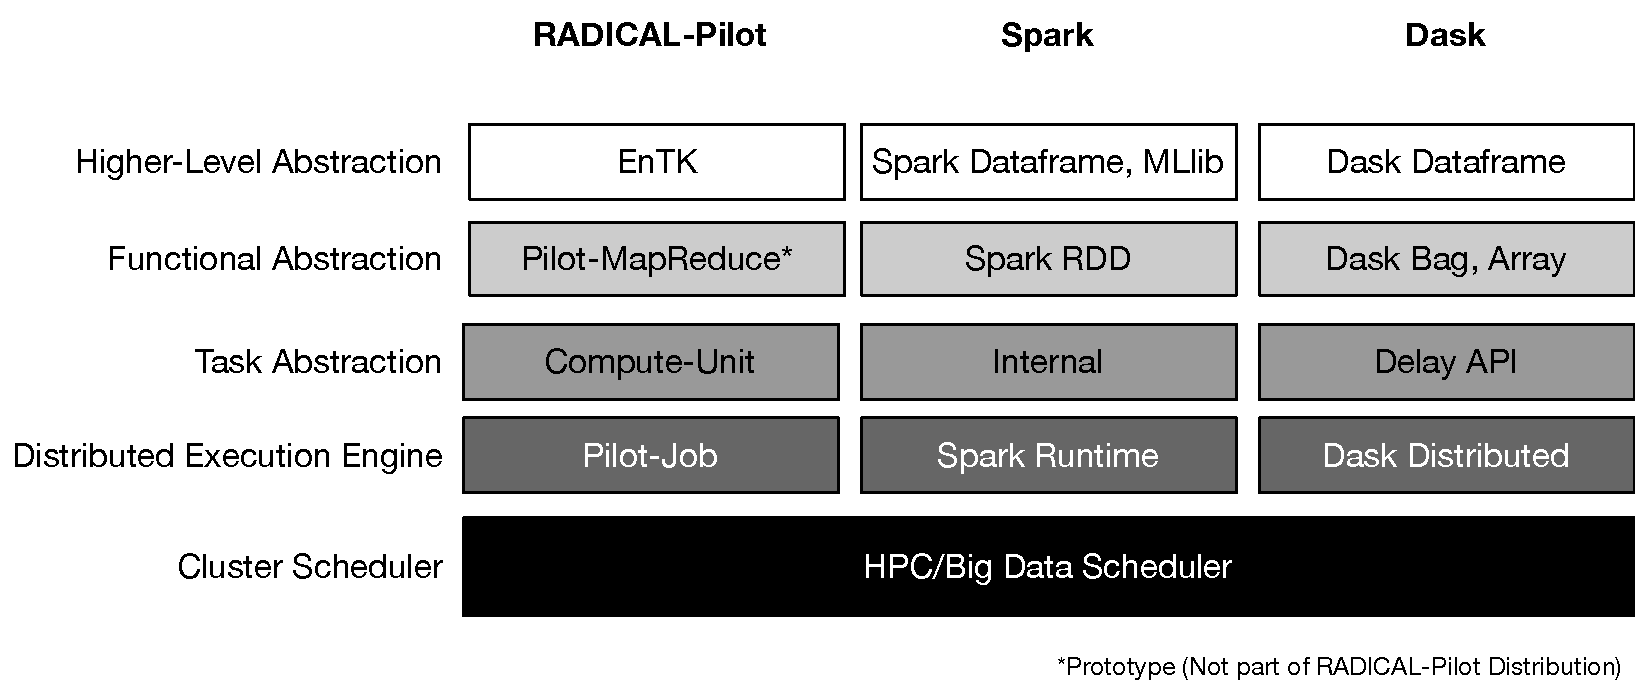
\includegraphics[width=.95\textwidth]{figures/data_analytics_hpc/task_par/bigdata_framework_stack.pdf}
    \caption{Architecture of RADICAL-Pilot, Spark and Dask.}
    %\caption{\textbf{Architecture of RADICAL-Pilot, Spark and Dask:}
    %The frameworks share common architectural components for managing cluster resource, and tasks.
    %Spark, Dask offer several high-level abstractions inspired by MapReduce.}
    \label{fig:figures_bigdata_framework_stack}
\end{figure}

\subsubsection*{RADICAL-Pilot}

%RADICAL-Pilot~\cite{merzky2019using} is a Pilot system that implements the
%pilot paradigm as outlined in Ref.~\cite{turilli2018comprehensive}.
%RADICAL-Pilot (RP) is implemented in Python and provides a well defined API and
%usage modes. Although RP is vehicle for research in scalable computing, it also
%supports production grade science. Currently, it is being used by applications
%drawn from diverse domains, ranging from earth and biomolecular sciences to
%high-energy physics. RP can be used as a runtime system by workflow or workload
%management
%systems~\cite{turilli2019middleware,treikalis2016repex,balasubramanian2018harnessing,dakka2018high,turilli2017evaluating}.
%In 2017, RP was used to support more than 100M core-hours on US DOE, NSF
%resources (BlueWaters and XSEDE), and European supercomputers (Archer and
%SuperMUC).

As discussed in~\S\ref{ch:pilot-data-hadoop}, RP allows concurrent
task execution on HPC resources. The user defines a set of Compute-Units (CU)
which are submitted to RP. RP schedules these CUs for
execution on the acquired resources and uses the existing environment of the
resource to execute tasks. Any data communication between tasks is done via an
underlying shared filesystem, e.g., Lustre. Task execution coordination and
communication is done through a database (MongoDB).

%RP's learning curve can be quite steep at the beginning, at least
%until the user becomes familiar with the concept and usability of Pilots and
%CUs. Once the user is comfortable with RP's API, she can easily
%develop new algorithms.

\subsubsection*{Spark}

Spark~\cite{zaharia2010spark} extends MapReduce~\cite{dean2004mapreduce},
providing a rich set of operations on top of the Resilient Distributed Dataset
(RDD) abstraction~\cite{zaharia2012resilient}. RDDs are cached in-memory, making
Spark well suited for iterative applications that need to cache a set of data
across multiple stages. PySpark provides a Python API to Spark.

A Spark workflow consists of multiple stages. Each stage is a set of independent
parallel tasks (e.g., \texttt{map}) and an action (e.g., \texttt{reduce}).
Spark's Scheduler translates the workflow specified via RDD transformations and
actions to an execution plan. Its distributed execution engine handles the
low-level details of task execution, which is triggered by actions. Spark can
read data from different sources, such as HDFS, blob storage, parallel and local
filesystems. Spark offloads data to disk when there is not enough free memory
on a node. Persisted RDDs remain in memory,
unless specified to use the disk either complementary or as a single target. In
addition, Spark writes data that are used in a shuffle to disk. As a result, Spark
allows quick access to those data when transmitted to an executor.
%Finally, Spark provides a set of actions that write text files, Hadoop sequence files or object files to local filesystems, HDFS or any filesystem that supports Hadoop.
%In addition, Spark supports higher-level data abstractions for processing structured data, such as dataframes, Spark-SQL, datasets, and data streams.

\subsubsection*{Dask}

Dask~\cite{rocklin2015dask} provides a Python-based parallel computing library,
which is designed to parallelize native Python code written for NumPy and
Pandas. In contrast to Spark, Dask also provides a lower-level task API
(\texttt{delayed} API) that allows users to construct arbitrary workflow graphs.
Being written in Python, it does not require to translate data types from one
language to another like PySpark, which moves data between Python's interpreter
and Java/Scala.

In addition to the low-level task API, Dask offers three higher-level
abstractions: Bags, Arrays and Dataframes. Dask Arrays are a collection of NumPy
arrays organized as a grid. Dask Bags are similar to Spark RDDs and are used to
analyze semi-structured data, like JSON files. Dask Dataframes are distributed
collections of Pandas dataframes that can be analyzed in parallel.

Dask also offers three schedulers: multithreading, multiprocessing and
distributed. The multithreaded and multiprocessing schedulers support only
single node execution and the parallel execution is done via threads and processes
respectively. The distributed scheduler creates a cluster with a scheduling
process and multiple worker processes. A client process creates and communicates
a workflow as a direct acyclic graph to the scheduler. Finally, the scheduler
assigns tasks to workers.

%Dask's learning curve cannot be considered steep. Its API is well defined and
%documented. In addition, familiarity with Spark or MapReduce helps to minimize
%the learning curve even further. As a result, implementing MD analysis
%algorithms on Dask did not require significant engineering time. In addition,
%setting up a Dask cluster on a set of resources was relatively straightforward,
%since it provides all the binaries, e.g. \texttt(dask-ssh).

%\subsubsection*{RP} RP~\cite{merzky2019using} is a Pilot
%system that implements the pilot paradigm as outlined in
%Ref.~\cite{turilli2018comprehensive}. RP (RP) is implemented in
%Python and provides a well defined API and usage modes. Although RP is vehicle
%for research in scalable computing, it also supports production grade science.
%Currently, it is being used by applications drawn from diverse domains, ranging
%from earth and biomolecular sciences to high-energy physics. RP can be used as
%a runtime system by workflow or workload management
%systems~\cite{turilli2019middleware,treikalis2016repex,balasubramanian2018harnessing,dakka2018high,turilli2017evaluating}.
%In 2017, RP was used to support more than 100M core-hours on US DOE, NSF
%resources (BlueWaters and XSEDE), and European supercomputers (Archer and
%SuperMUC).

%RP allows concurrent task execution on HPC resources. The user
%defines a set of Compute~-Units (CU)~- the abstraction that defines a task
%along with its dependencies - which are submitted to RP.
%RP schedules these CUs to be executed under the acquired resources.
%It uses the existing environment of the resource to execute tasks. Any data
%communication between tasks is done via an underlying shared filesystem, e.g.,
%Lustre. Task execution coordination and communication is done through a
%database (MongoDB).

%RP's learning curve can be quite steep at the beginning, at least
%until the user becomes familiar with the concept and usability of Pilots and
%CUs. Once the user is comfortable with RP's API, she can easily
%develop new algorithms.

\subsection{Comparison}
\begin{table}[t]
    \scriptsize
    \centering
    \begin{tabular}{@{}p{2.75cm}|p{3.25cm}p{3.25cm}p{3.25cm}@{}}
        \toprule
        &\textbf{RADICAL-Pilot} &
        \textbf{Spark} &
        \textbf{Dask} \\
        \midrule
        % row 1
        Languages &
        Python &
        Java, Scala, Python, R &
        Python\\
        % Row 2
        Task &
        Task &
        Map-Task &
        Delayed\\
        % row 3
        Abstraction &
        &
        & \\
        % row 4
        Functional Abstraction  &
        - &
        RDD API &
        Bag\\
        % row 5
        Higher-Level Abstractions &
        Pipelines~\cite{balasubramanian2018harnessing}, Replicas~\cite{dakka2018concurrent} &
        Dataframe, ML Pipeline, MLlib~\cite{meng2016mllib} &
        Dataframe, Arrays for block computations\\
        % row 6
        Resource Management &
        Pilot-Job &
        Spark Execution Engines &
        Dask Distributed Scheduler\\
        % row 7
        Scheduler    &
        Individual Tasks &
        Stage-oriented DAG &
        DAG\\
        % row 8
        Shuffle      &
        -       &
        hash/sort-based shuffle &
        hash/sort-based shuffle\\
        % row 8
        Limitations &
        no shuffle, filesystem-based communication  &
        high overheads for Python tasks (serialization)   &
        Dask Array can not deal with dynamic output shapes\\
        \bottomrule
    \end{tabular}
    \caption{Task-parallel Frameworks Comparison.\label{tab:frameworks}}
    %\caption{\textbf{Task-parallel Frameworks Comparison:} Dask and Spark are designed for data-related task, while RADICAL-Pilot focuses on compute-intensive tasks.\label{tab:frameworks}}
\end{table}

Table~\ref{tab:frameworks} summarizes the properties of Spark, Dask and
RP with respect to the abstractions and runtime systems provided to
create and execute parallel data applications.

\subsubsection*{API and Abstractions}

RP provides a low-level API for executing tasks onto resources. While
this API can be used to implement high-level capabilities, e.g.,
MapReduce~\cite{mantha2012pilot}, they are not provided out-of-the box. Both
Spark and Dask provide such capabilities. Dask's API is generally lower level
than Spark's, i.e., it allows specifying arbitrary task graphs. Although Spark
decides the partition size automatically, in many cases it is necessary to tune
parallelism by specifying the number of partitions.

Another important aspect is the availability of high-level abstractions.
High-level abstractions for RP, such as
Pipelines~\cite{balasubramanian2018harnessing} and
Replicas~\cite{dakka2018concurrent}, support compute-oriented
tasks and workflows. Contrary, Spark and Dask already offer a set of
high-level data-oriented abstractions, such as Dataframes.

%\mtnote{I am not sure
%those are a valid comparisons: high-level abstraction Vs. tools; dataframes Vs.
%workflows. I would eliminate tools, using only abstractions. I would then
%compare DataFrame to Pipelines, possibly adding Replicas and a reference to
%HTBAC.}

\subsubsection*{Scheduling}

Both Spark and Dask create a Direct Acyclic Graph (DAG) based on operations over
data, which their respective execution engine executes. Spark jobs are
separated into stages. When a stage finishes, the scheduler executes the
next stage.

Dask's DAGs have a tree representation where each node is a task. Leaf tasks do
not depend on other task for execution. Dask tasks execute when their
dependencies are satisfied, starting from leaf tasks. When the scheduler reaches a task
with unsatisfied dependencies, the scheduler executes the dependent task first.
Dask's scheduler does not rely on synchronization points that Spark's
stage-oriented scheduler introduces. RP does not provide a DAG-based
API and requires the user to manage the execution order and synchronization
among tasks at application level instead of runtime level (i.e., RP).

\subsection{Frameworks Evaluation}
\label{sec:framework_eval}

As data-parallelism often involves a large number of short-running tasks, task
throughput is a critical metric to assess the three frameworks we consider. To
evaluate the throughput of those frameworks, we use zero workload tasks
(\texttt{/bin/hostname}). We submit an increasing number of such tasks to
RP, Spark and Dask and measure the execution time on a single node.

For RP, all tasks were submitted simultaneously. RP's
backend database was running on the same node to avoid communication
latencies. For Spark, we created an RDD with as many partitions as the number of
tasks, as each task maps to a partition by Spark. For Dask, we created tasks
using \texttt{delayed} functions that were executed by the Distributed
scheduler. We used TACC Wrangler and SDSC Comet for this experiment. SDSC Comet
is a 2.7 petaFLOSP cluster with 24 Haswell cores/node and 128\,GB memory/node
(6,400 nodes). TACC Wrangler has 24 Haswell hyper-threading enabled cores/node
and 128\,GB memory/node (120 nodes).

\begin{figure}[t]
    \centering
    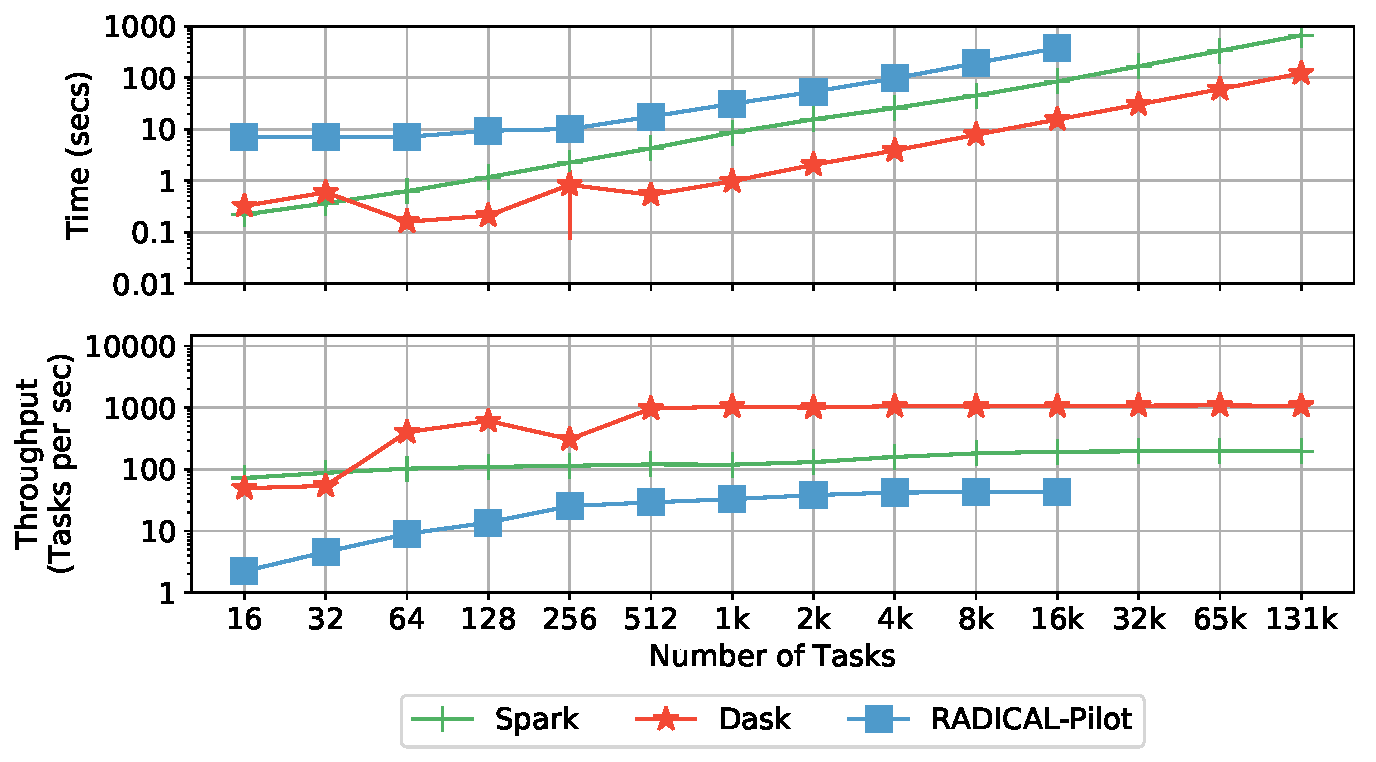
\includegraphics[width=.75\textwidth]{figures/data_analytics_hpc/task_par/dask_spark_rp_wrangler.pdf}
    \caption{Total time to completion and task throughput by framework on a
    single node for an increasing number of tasks on Wrangler.}
    \label{fig:dask_spark_rp_wrangler}
\end{figure}

Figure~\ref{fig:dask_spark_rp_wrangler} shows the total time to completion and
task throughput. Dask needed the least time to schedule and execute the assigned
tasks, followed by Spark and RP. Dask and Spark quickly reach their
maximum throughput, which is sustained as the number of tasks increased.
RP showed the worst throughput and scalability, mainly due to some
architectural limitations. Specifically, RP relies on a MongoDB
database to communicate between Client and Agent, as well as several components
that allow RP to move data and introduce delays in the execution of
the tasks. As a result, we were not able to scale RP to 32k or more
tasks.

\begin{figure}[t]
    \centering
    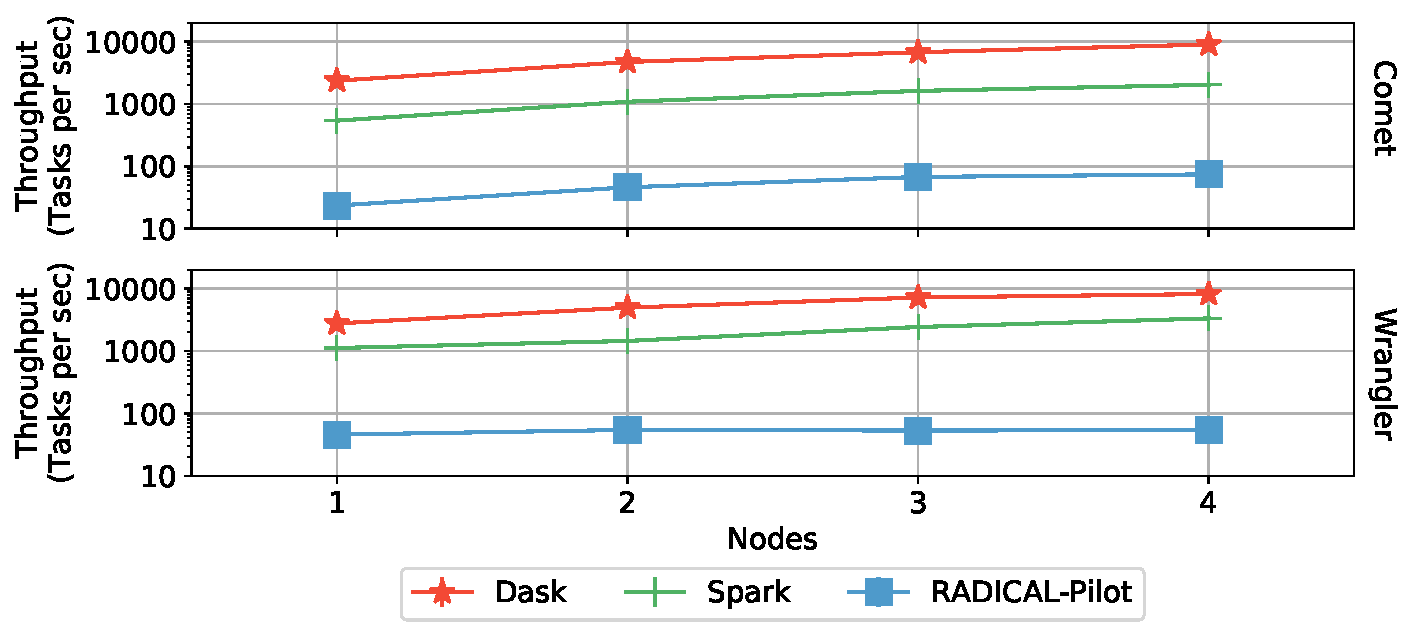
\includegraphics[width=.75\textwidth]{figures/data_analytics_hpc/task_par/daskVSsparkVSRpThroughput.pdf}
    \caption{Task throughput by framewrork for $100k$ tasks on different number of nodes.}
    \label{fig:RP_Dask_Spark_throughput}
\end{figure}

Figure~\ref{fig:RP_Dask_Spark_throughput} illustrates task throughput when
scaling to multiple nodes, measured by submitting $100k$ tasks. Dask's
throughput on both resources increases almost linearly to the number of nodes.
Spark's throughput is an order of magnitude lower than Dask's. RP's
throughput plateaus below $100 task/sec$. Wrangler and Comet show a comparable
performance, with Comet slightly outperforming Wrangler.

%\subsubsection*{Suitability for MDAnalysis Algorithms} Trajectory analysis
%methods are often embarrassingly parallel. So, they are ideally suited for task
%management and MapReduce APIs. PSA-like methods typically require a single pass
%over the data and return a set of values that correspond to a relationship
%between frames or trajectories. They can be expressed as a bag of tasks using a
%task management API or a map-only application in a MapReduce-style API.

%Leaflet Finder is more complex and requires two stages: \begin{inparaenum}[a)]
%\item the edge discovery stage, and \item the connected components stage.
%\end{inparaenum} It is possible to implement Leaflet Finder with a simple
%task-management API, although the MapReduce programming model allows more
%efficient implementation with a \texttt{map} for computing and filtering
%distances and a \texttt{reduce} for finding the components. The shuffling
%required between map and reduce is medium as the number of edges is a fraction
%of the input data.

\section{Task-Parallel MD Trajectory Data Analysis: Implementation \& Characterization}
\label{sec:impl_exp}

In this section, we characterize and evaluate the performance of two algorithms
from MDAnalysis---PSA and LF---using different real-world datasets,
when implemented with RP, Spark and Dask. We compare the performance
of these three task-parallel frameworks with an equivalent implementations of
the algorithms using MPI4py. We investigate:
\begin{inparaenum}[1)]
    \item which capabilities and abstractions of the frameworks are needed to
    efficiently express these algorithms;
    \item what architectural approaches can be used to implement these
    algorithms with these frameworks; and
    \item the performance trade-offs of these frameworks.
\end{inparaenum}

The experiments were executed on SDSC Comet and TACC Wrangler. Experiments were
carried using RP and Pilot-Spark (as discussed
on~\S\ref{ch:pilot-data-hadoop}). We utilize a set of custom scripts to start
the Dask cluster. We used RP 0.46.3, Spark 2.2.0, Dask 0.14.1 and
Distributed 1.16.3.
%The data presented are means over multiple runs; error bars represent the
%standard deviation of the sample.
We employed up to $10$ nodes on Comet and Wrangler.

\subsection{Path Similarity Analysis (PSA): Hausdorff Distance}
\label{sec:psa}

The PSA algorithm is embarrassingly parallel and can be implemented using simple
task-level parallelism or a map-only MapReduce application. We equally distribute
the input data, i.e., a set of trajectory files, over the cores,
generating one task per core. Each task reads its respective input files in
parallel, executes and writes the result to a file.

For RP, we define a CU for each task and execute them using
a Pilot-Job. For Spark, we create an RDD with one data partition per task which
is a \texttt{map} function. In Dask, tasks are defined as
\texttt{delayed} functions and in MPI, each task is executed by an MPI process.
The dataset used for the experiments consists of three atom count trajectories:
\begin{inparaenum}[1)]
    \item small (3341 atoms/frame);
    \item medium (6682 atoms/frame); and
    \item large (13364 atoms/frame).
\end{inparaenum}
We used 102 frames, and 128 and 256 trajectories of each size.

Figure~\ref{fig:HausdorffWrangler} shows the runtime for 128 and 256
trajectories on Wrangler, while Figure~\ref{fig:comet_wrangler_haus} compares
the execution times on Comet and Wrangler for 128 large trajectories. The
three frameworks show similar performance in terms of runtime on both systems,
as well as with MPI4py. Wrangler gives smaller speedup than Comet
despite using the same number of cores. Wrangler uses hyperthreading and, as a
result, multiple tasks share the same CPU, resulting in lower speedup than
Comet.

\begin{figure}[t]
    \centering
    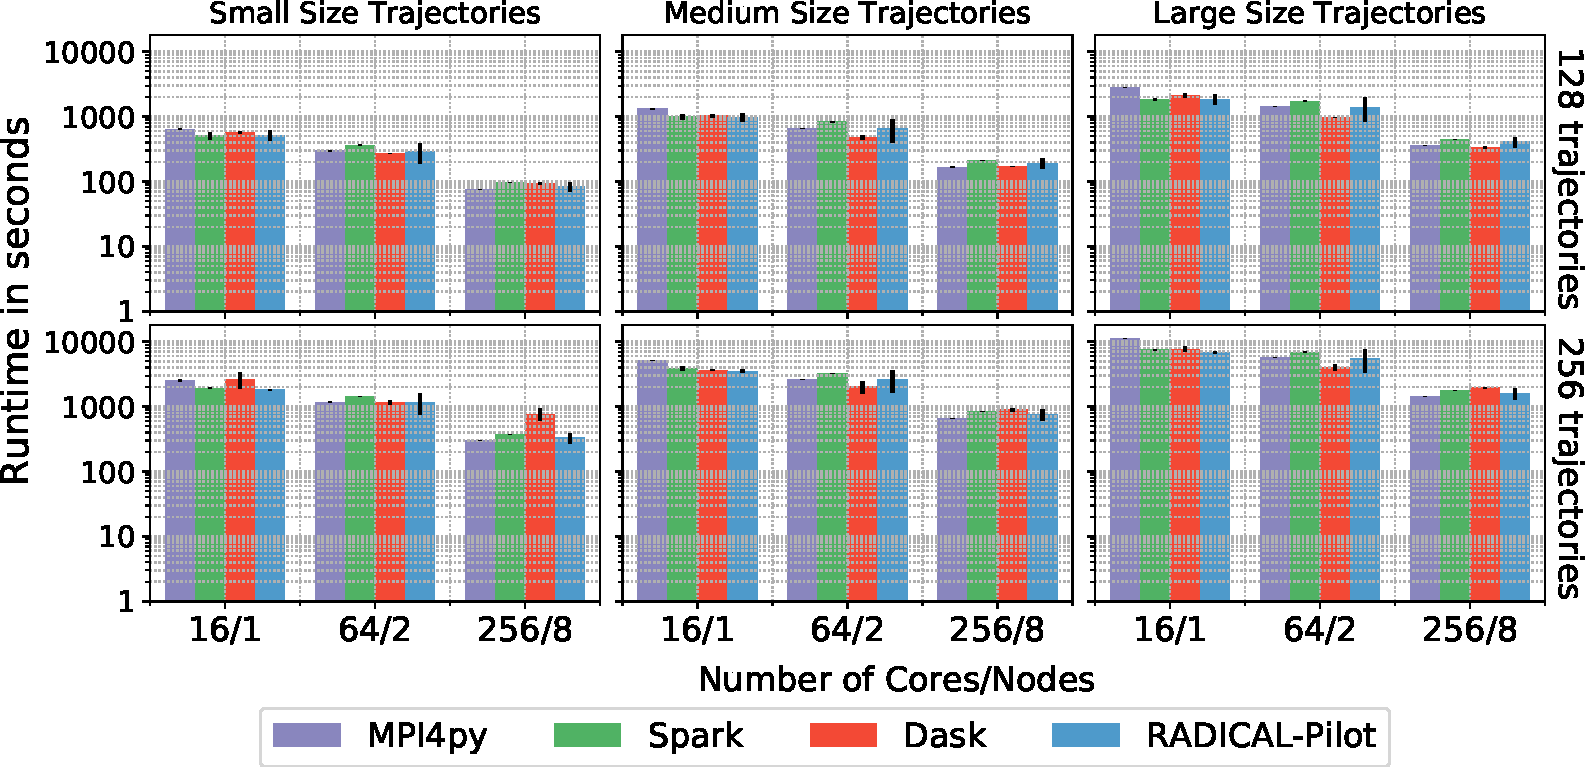
\includegraphics[width=0.85\textwidth]{figures/data_analytics_hpc/task_par/HausdorffSingleFig.pdf}
    \caption{Time to completion of PSA on Wrangler using RADICAL-Pilot, Spark
    and Dask over different number of cores, trajectory sizes, and number of
    trajectories.}
    \label{fig:HausdorffWrangler}
\end{figure}

\begin{figure}[t]
    \centering
    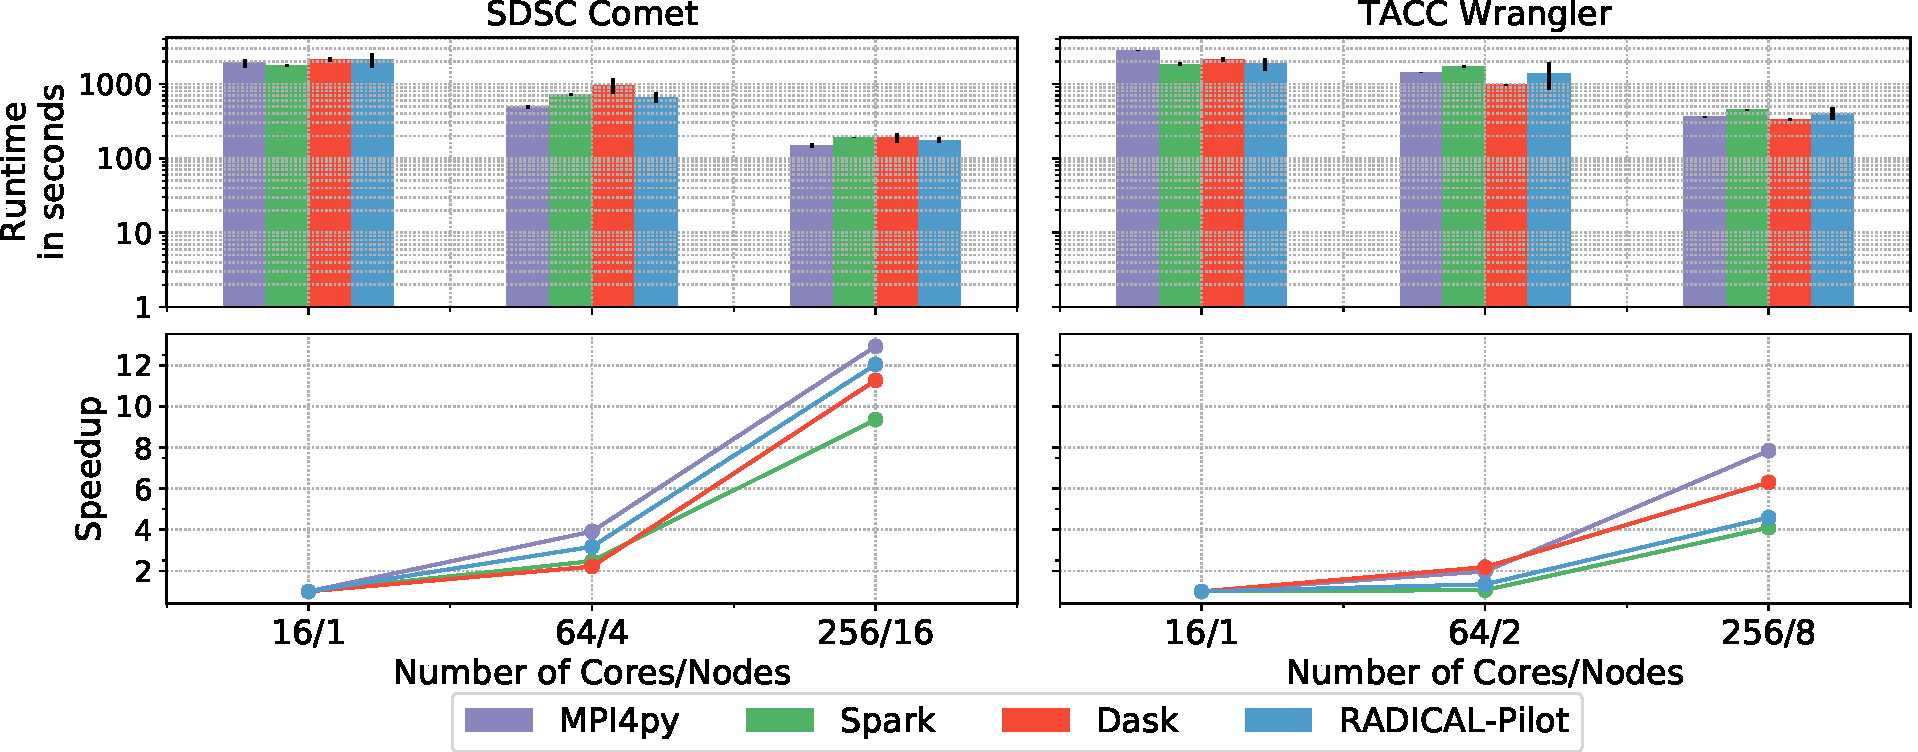
\includegraphics[width=.85\textwidth]{figures/data_analytics_hpc/task_par/comet_wrangler_haus.pdf}
    \caption{Time to completion and speedup of PSA on Comet and Wrangler for 128 large trajectories.}
    \label{fig:comet_wrangler_haus}
\end{figure}

MPI4py, RP, Spark and Dask have similar performance when used to
execute embarrassingly parallel algorithms. All frameworks achieved similar
speedups as the number of cores increased, scaling by a factor of 6 from 16 to
256 cores, which are lower than MPI4py. Although the frameworks' overheads are
comparably low in relation to the overall runtime, the overheads were significant
enough to impact the frameworks' speedup. Note that RP's large
deviation is due to sensitivity to communication delays with the database.

In summary, for embarrassingly parallel algorithms all three frameworks provide
appropriate abstractions and runtime performance compared to MPI. Beyond
performance considerations, aspects such as programmability and
integrate-ability are more important considerations when comparing the three
frameworks. Both RP and Dask are native Python frameworks, making the
integration with other Python tools easier and more efficient than with
frameworks which are based on other languages like Spark.

\subsection{Leaflet Finder (LF)}
\label{sec:leaflet}

\begin{table*}[t]
    \scriptsize
    \centering
    \begin{tabular}{@{}p{2cm}|p{2.8cm}p{2.8cm}p{2.8cm}p{2.8cm}@{}}
        \toprule
        &
        \textbf{Broadcast and 1-D} (Approach 1) &
        \textbf{Task API and 2-D} (Approach 2) &
        \textbf{Parallel Connected Components} (Approach 3) &
        \textbf{Tree-Search} (Approach 4)\\
        \midrule
        % row 1
        Data Partitioning  &
        1D  &
        2D &
        2D &
        2D\\
        % row 2
        Map &
        Edge Discovery via Pairwise Distance &
        Edge Discovery via Pairwise Distance &
        Edge Discovery via Pairwise Distance and Partial Connected Components &
        Edge Discovery via Tree-based Algorithm and Partial Connected Components\\
        % row 3
        Shuffle &
        Edge List ($O(E)$) &
        Edge List ($O(E)$) &
        Partial Connected components ($O(n)$) &
        Partial Connected components ($O(n)$)\\
        % row 4
        Reduce   &
        Connect Components  &
        Connected Components &
        Joined Connected Components &
        Joined Connected Components\\
        \bottomrule
    \end{tabular}
    \caption{MapReduce Operations used by Leaflet Finder\label{tab:app_operators}}
\end{table*}

\begin{figure*}[t]
    \centering
    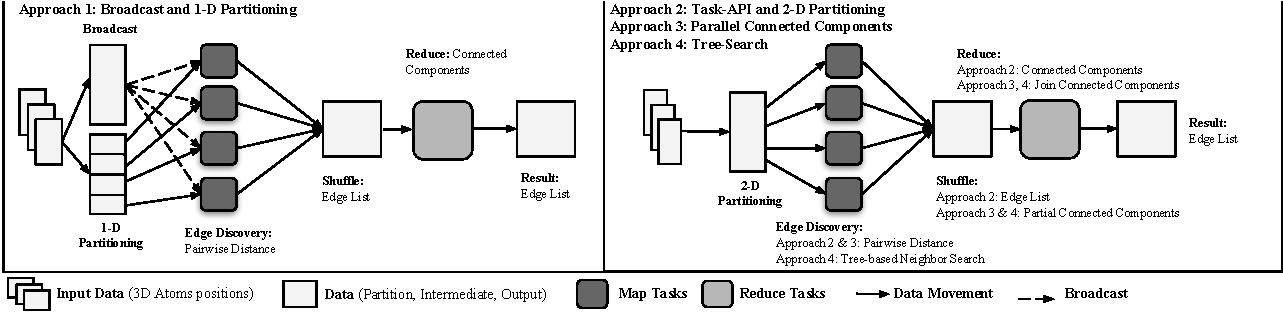
\includegraphics[width=.95\textwidth]{figures/data_analytics_hpc/task_par/lf_approaches.pdf}
    \caption{Architectural approaches for implementing the Leaflet finder algorithm\label{fig:lf_approaches}}
\end{figure*}

We developed five approaches to implement the LF algorithm using RP,
Spark, Dask, and MPI4py (see Fig~\ref{fig:lf_approaches} and
Table~\ref{tab:app_operators}):
\begin{enumerate}[1)]
    \item \textbf{Broadcast and 1-D Partitioning:} Broadcast and partition
    through a data abstraction the physical system. Use of RDD API
    (broadcast), Dask Bag API (scatter), and MPI Bcast to distribute data to all
    nodes. A \texttt{map} function calculates the edge list using \texttt{cdist}
    from SciPy~\cite{scipy}, realized as a loop for MPI. The master process (rank 0)
    collects (gathers) the list and calculates the connected components.\label{en:1}
    \item \textbf{Task API and 2-D Partitioning:} Data management is done
    without using the data-parallel API. The framework is used for task
    scheduling. Data are pre-partitioned in 2-D partitions and passed to a
    \texttt{map} function that calculates the edge list using \texttt{cdist},
    realized as a loop for MPI.  The master process (rank 0)
    collects (gathers) the list and calculates the connected components.\label{en:2}
    \item \textbf{Parallel Connected Components:} Data are managed as in
    approach~\ref{en:2}. Each \texttt{map} task performs edge list and connected
    components computations. The reduce phase joins the calculated components
    into one, when there is at least one common node.\label{en:3}
    \item \textbf{Tree-based Nearest Neighbor and Parallel-Connected Components
    (Tree-Search):} This approach is different to approach~\ref{en:3} only for
    the way in which edge discovery is implemented in the \texttt{map} phase. A
    tree containing all atoms is created which is then used to query for
    adjacent atoms.\label{en:4}
\end{enumerate}

We use four physical systems with 131k, 262k, 524k, and 4M atoms with
896k, 1.75M, 3.52M, and 44.6M edges in their graphs. We utilized up to
256 cores on Wrangler for our experiments. Data partitioning results into 1024
partitions for each approach, thus 1024 \texttt{map} tasks. Due to memory
limitations from using \texttt{cdist} -- uses double precision floating point --
Approach \ref{en:3} data partitioning of the 4M atom dataset resulted to 42k
tasks for both Spark and MPI4py.

Figure \ref{fig:All4approachesNoRp} shows the runtimes for all datasets for
Spark, Dask and MPI4py. Figure~\ref{fig:rpLF} shows RP's performance.
 We continue by analyzing the performance of each
architectural approach and used framework in detail.

\begin{figure}[t]
    \centering
    \begin{subfigure}{.85\textwidth}
        \centering
        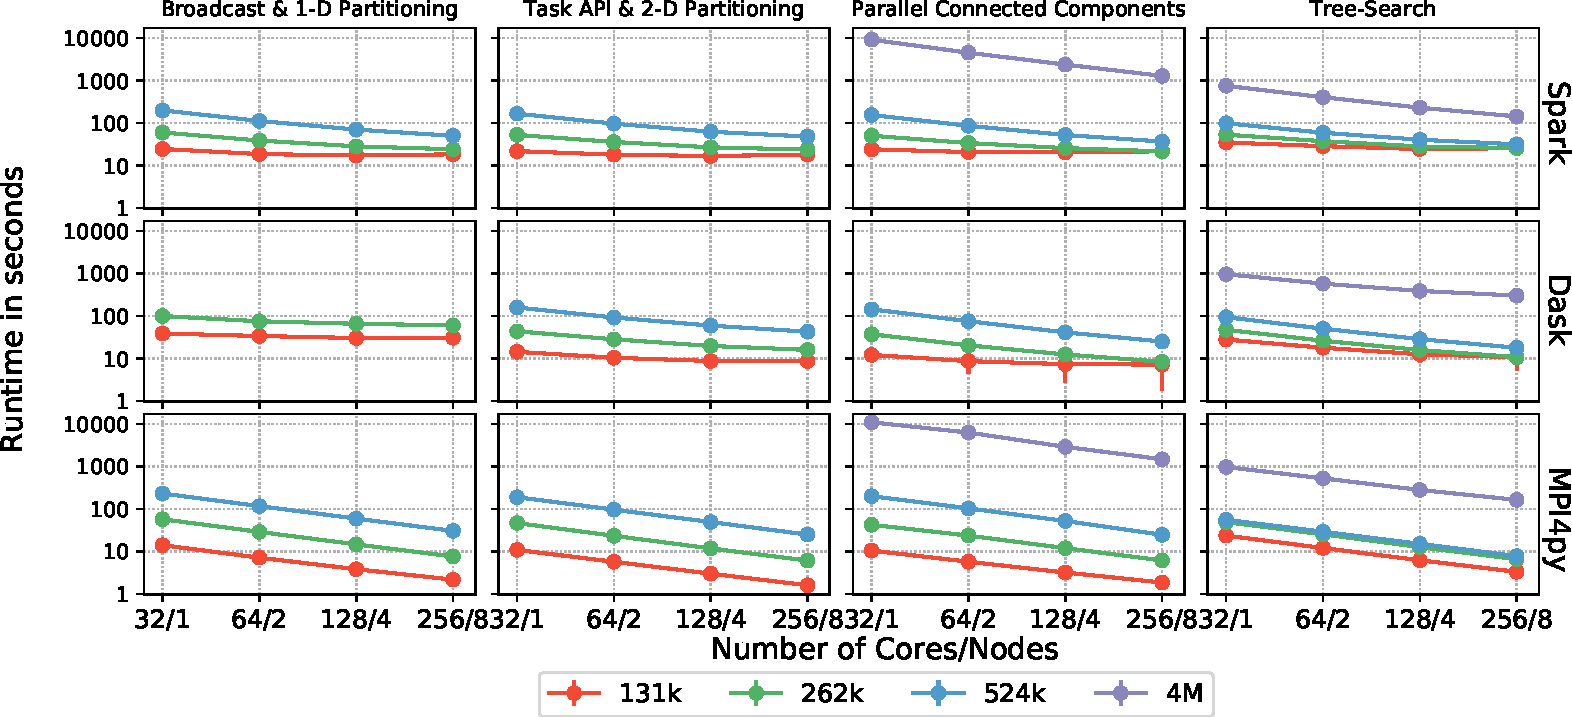
\includegraphics[width=.95\linewidth]{figures/data_analytics_hpc/task_par/All4approachesWith4M_logscaleline.pdf}
    \end{subfigure}\\
    \begin{subfigure}{.85\textwidth}
        \centering
        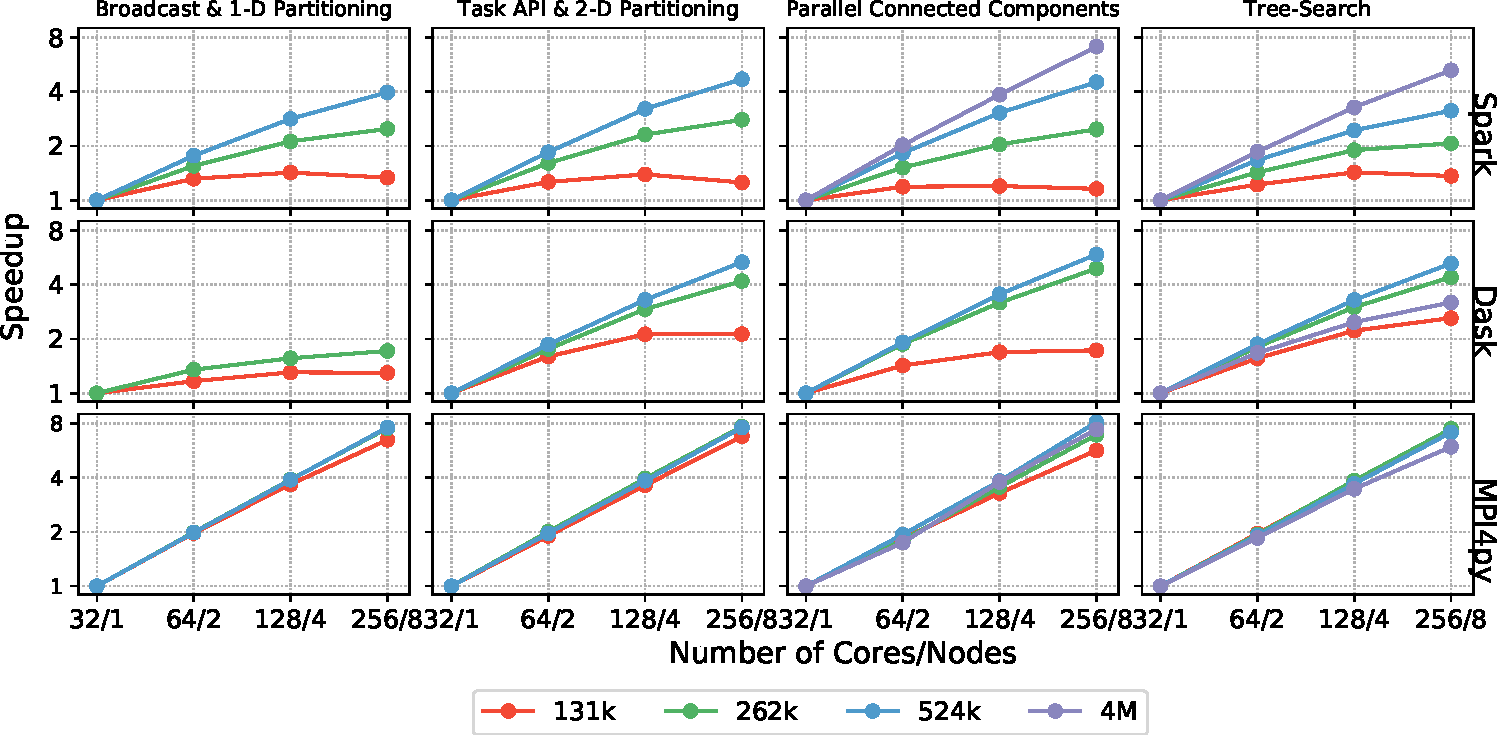
\includegraphics[width=.95\linewidth]{figures/data_analytics_hpc/task_par/All4approachesWith4MSpeedup.pdf}
    \end{subfigure}
    \caption{Leaflet Finder Performance of Different Architectural Approaches
            for Spark \& Dask. Runtimes and Speedups for different system sizes
            over different number of cores for all approaches and frameworks.}
    \label{fig:All4approachesNoRp}
\end{figure}

%%%%%%%%%%%%%%% APPROACH 1 %%%%%%%%%%%%%%%%%%
\subsubsection*{Broadcast and 1-D Partitioning}

Approach 1 broadcasts data to nodes via the capabilities supported by Spark,
Dask and MPI. All nodes maintain a complete copy of the dataset and each
\texttt{map} task computes the pairwise distance on a partition of the dataset.
%\mtnote{its
%partition of what? Note: 'its', 'it' and 'they' in English should not be used
%when it is not clear to what subject or complement they refers, especially at
%the beginning of a sentence. I have been correcting tens of those so far. In
%this sentence, it is not possible to understand to what 'its' referes: to the
%task, to the node, to the broadcast?}
%We use 1-D partitioning.
Figure~\ref{fig:WranglerLeafLetFinderApp1} shows the detailed results.

\begin{figure}[t]
    \centering
    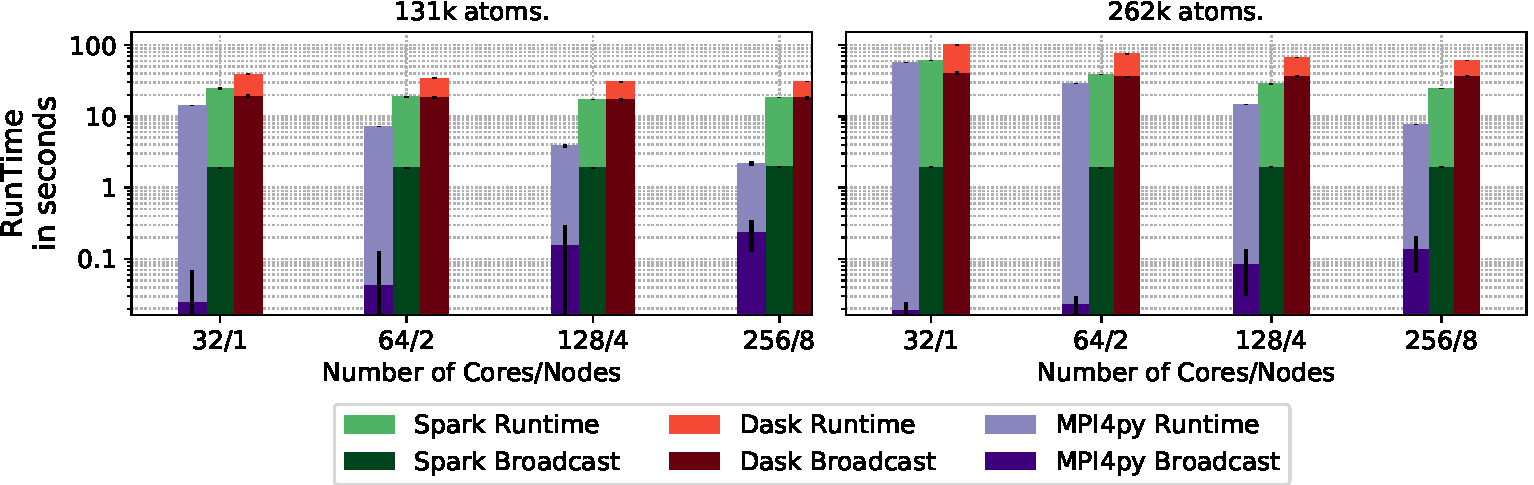
\includegraphics[width=.75\textwidth]{figures/data_analytics_hpc/task_par/spark_dask_lf_approach1.pdf}
    \caption{Broadcast and 1-D Partitioned Leaflet Finder (Approach 1). Runtime
    for multiple system sizes on different number of cores for Spark, Dask and
    MPI4py.}
    \label{fig:WranglerLeafLetFinderApp1}
\end{figure}

The usage of broadcast capabilities has severe limitations for Spark and Dask.
MPI broadcast is a fraction of the overall execution time and significantly
smaller than Spark and Dask. MPI's broadcast times increase linearly as the
number of processes increases, while Spark's and Dask's remain relatively
constant for each dataset, due to more elaborate broadcast algorithms compared
to MPI. Broadcast times are between 3\% and 15\% of the edge discovery time
for Spark, from 40\% to 65\% for Dask, and from <1\% to 10\% for MPI4py.
Thus, Spark offers a more efficient communication subsystem compared to Dask. In
addition, Dask broadcast partitions the dataset to a list where each element
represents a value from the initial dataset. This did not allow broadcasting the
524k atom dataset. Nevertheless, the limited scalability of this approach due
to transmitting the entire dataset makes it usable only for small datasets.

Using broadcast shows the worst performance and scaling of all approaches for
Spark, Dask and MPI4py. This approach scales only up to 262k atoms for Dask,
and 524k atoms for Spark and MPI4py on Wrangler. Spark's performance is
comparable to MPI4py for the 262k, and 524k datasets. Spark
also shows better performance
for the smallest core count in the 524k case. Dask is at least two times
slower than our MPI implementation.

%%%%%%%%%%%%%%% APPROACH 2 %%%%%%%%%%%%%%%%%%
\subsubsection*{Task-API and 2-D Partitioning}

Approach~\ref{en:2} tries to overcome the limitations of approach 1, especially
broadcasting and 1-D partitioning. A 2-D block partitioning evenly distributes
the compute and utilizes  more efficiently the available memory.
Spark and Dask do not support well 2-D partitioning. Spark's RDDs
are optimized for data-parallel applications with 1-D partitioning. While Dask's
array supports 2-D block partitioning, it was not used for this implementation.
We return the adjacency list of the graph instead of an array to fully use the
capabilities of the abstraction. Thus, each task works on a 2-D pre-partitioned
part of the input data.

Figure~\ref{fig:All4approachesNoRp} shows the runtimes of approach~\ref{en:2}
for Spark, Dask, and MPI4py, and Figure~\ref{fig:rpLF} shows the runtime of
approach~\ref{en:2} for RP. As expected, this approach overcomes the
limitations of approach 1 and can easily scale to larger datasets (e.g., 524k
atoms) while improving the overall runtime. Dask's execution time was smaller by
at least a factor of two compared to
approach 1. However, we were not able to scale this implementation to the 4M
dataset due to the memory requirements of \texttt{cdist}. For RP, we
observed significant task management overheads (see also
section~\ref{sec:framework_eval}). This is a limitation of RP with
respect to managing large numbers of tasks, particularly visible when running on
a single node with 32 cores. As more than 64 cores become available,
RP's performance improves dramatically.

\begin{figure}[t]
    \centering
    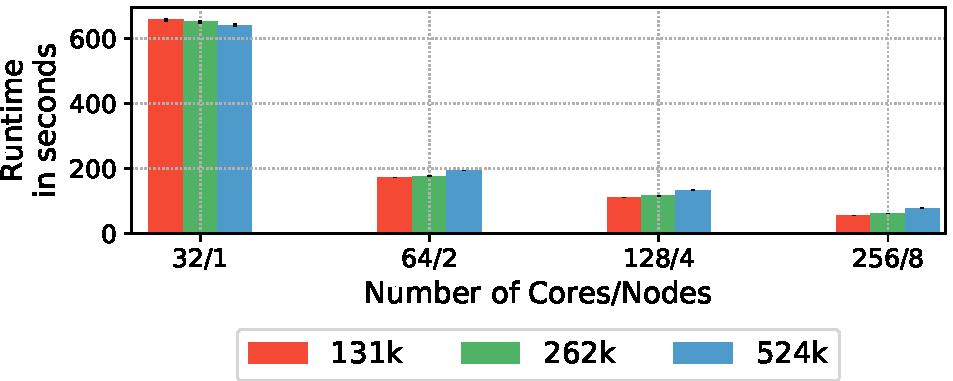
\includegraphics[width=.75\textwidth]{figures/data_analytics_hpc/task_par/rpLF.pdf}
    \caption{RADICAL-Pilot Task API and 2-D Partitioned Leaflet Finder (Approach
    2). Runtime for multiple system sizes over different number of cores.}
    %Overheads dominate since execution times are similar despite the system size.}
    \label{fig:rpLF}
\end{figure}

Spark and Dask did not scale as well as MPI, which achieved linear speedups of
$\sim8$ when using 256 cores. Spark and Dask achieved maximum speedups of
$4.5$ and $\sim5$ respectively. Despite this fact, both frameworks had similar
performance on 32 cores for the 262k and 524k datasets.

%%%%%%%%%%%%%% Approach 3 %%%%%%%%%%%%%%%%%%%%%%%
\subsubsection*{Parallel Connected Components}

Communication between the edge discovery and connected components phases is
another important aspect. For the 524k atoms dataset, the output of the edge
discovery phase is $\approx$ $100\,\textup{MB}$. To reduce the amount of data
that need to be shuffled, we refined the algorithm to compute the graph
components on the partial dataset in the \texttt{map} phase. The \texttt{reduce}
phase then merges the components. This reduces the amount
of shuffle data by more than 50\% (e.g., to 12\textup{MB} for Spark and
48\textup{MB} for Dask). Figure~\ref{fig:All4approachesNoRp} shows the
improvements in runtime, by $\sim20\%$ for Spark and Dask, but not MPI4py.
Further, we were able to run very large datasets, such as the 4M dataset, using
this architectural approach only with Spark and MPI4py. Dask was restarting its
worker processes because their memory utilization was reaching 95\%.

Spark and Dask have comparable performance with MPI on 32 cores, which utilizes
a single node on Wrangler. However, while the MPI4py implementation scales
almost linearly for all datasets, Spark and Dask cannot, reaching a maximum of
$\sim5$ speedup for the three smaller datasets. In addition, Spark is able to scale
almost linearly for the 4M atoms dataset, providing comparable performance to
MPI4py.

%%%%%%%%%%%%%% Approach 4 %%%%%%%%%%%%%%%%%%%%%%%
\subsubsection*{Tree-Search}

A bottleneck of approaches~\ref{en:1},~\ref{en:2} and~\ref{en:3} is the edge
discovery via the naive calculation of the distances between all pairs of atoms.
In approach~\ref{en:4}, we replace the pairwise distance function with a
tree-based, nearest neighbor search algorithm, in particular
BallTree~\cite{omohundro89five}. The algorithm:
\begin{inparaenum}
    \item constructs of a tree; and
    \item queries for neighboring atoms.
\end{inparaenum}
Using tree-search, the computational complexity can be reduced from $n^2$ to
$log$. We use a BallTree as offered by Scikit-Learn~\cite{scikit-nearest} for
our implementation.

Figure \ref{fig:All4approachesNoRp} illustrates the performance of the
implementation. For small datasets, i.e., 131k and 262k atoms,
approach~\ref{en:3} is faster than the tree-based approach, since the number of
points is too small. For the large datasets, the tree approach is faster. In
addition, the tree has a smaller memory footprint than \texttt{cdist}.
As a result, the tree approach scaled to larger problems, e.g., a 4M atoms
and 44.6M edges dataset, without changing the total number of tasks.

Dask shows better scaling performance than Spark for 131k, 262k and 524k atoms. This
is not true for 4M atoms, indicating that Dask's communication layer is not
able to scale as well as Spark's one. Spark shows similar performance to MPI4py
for the largest dataset due to minimal shuffle traffic. Thus, MPI's efficient
communication does not become relevant.

\section{Conceptual Framework for Selecting Task-Parallel Frameworks}
\label{sec:task_sel_model}

In this section, we provide a conceptual framework that allows application
developers to select a framework according to their compute and I/O
requirements. It is important to understand the properties of both the
application and task-parallel frameworks. Table~\ref{tab:framework} illustrates
the criteria of this conceptual model and ranks the three frameworks.

\begin{table}[t]
    \scriptsize
    \centering
    \begin{tabular}{@{}cccc@{}}
        \toprule
        &\textbf{RADICAL-Pilot}     &\textbf{Spark} &\textbf{Dask}\\
        \multicolumn{4}{l}{\textbf{Task Management}} \\
        \midrule
        Low Latency   &- &o &+\\
        Throughput    &- &+ &++\\
        MPI/HPC Tasks &+ &o &o\\
        Task API   &+ &o &++\\
        Large Number of Tasks   &-- &++ &++\\\hline
        \multicolumn{4}{l}{\textbf{Application Characteristics}}\\\midrule
        Python/native Code &++ &o &+\\
        Java               &o &++ &o\\
        Higher-Level Abstraction &- &++ &+\\
        Shuffle                  &- &++ &+\\
        Broadcast                &- &++ &+\\
        Caching                  &- &++ &o\\
        \bottomrule
    \end{tabular}
    \caption{Task-parallel framework selection decision methodology: Criteria
        and Ranking for Framework Selection. -~: Unsupported or low performance
        +~: Supported, ++~: Major Support, and o~:Minor
        support.\label{tab:framework}}
\end{table}

%  application perspective
\subsubsection*{Application Perspective}

We showed that we can implement applications for MD trajectory data analysis
using Spark, Dask and RP, as well as MPI4py. Implementation aspects,
such as computational complexity, and shuffled data size greatly influence
performance. For embarrassingly parallel applications with coarse grained tasks,
such as PSA, the choice of the framework does not significantly influence
performance. In addition, the performance difference against MPI4py was not
significant
(Figures~\ref{fig:HausdorffWrangler},~\ref{fig:comet_wrangler_haus}). Thus,
aspects such as programmability and integrate-ability, become more important
than performance alone.

For fine-grained data parallelism, a data-parallel framework, such as Spark and
Dask, clearly outperforms RP
(Figures~\ref{fig:All4approachesNoRp},~\ref{fig:rpLF}). If there is coupling
between tasks, i.e., task communication is required, using Spark becomes
advantageous (Approaches~\ref{en:3} \& \ref{en:4}). MPI4py outperformed
Dask and Spark, despite both frameworks scaling for the larger datasets.
Especially Spark was able to provide linear speedup for approach~\ref{en:3} of
Leaflet Finder (Figure~\ref{fig:All4approachesNoRp}).

Integrating with frameworks that provide higher level abstractions provides
scalable solutions for more complex algorithms. However, integrating Spark with
other tools needs to be carefully considered. The integration of Python tools,
e.g., MDAnalysis, often causes overheads due to the frequent need for
serialization and copying data between the Python and Java space.

Dask has the smallest learning curve of all three frameworks. As a result, it
allows for faster prototyping compared to RP and Spark.
RP's learning curve is more steep, but is more versatile than Dask
and Spark, by offering the lowest level abstraction. Spark had the slowest
learning curve but it required tuning to get the number of tasks correctly, as
well as argument passing to map and reduce functions.

\subsubsection*{Framework Perspective}

RP is well suited for HPC applications, e.g., ensembles (up to $50k$
tasks) of parallel MPI applications, as shown in
Ref.~\cite{merzky2018design,merzky2019using}. It has limited scalability when
supporting large numbers of short-running tasks, as often found in
data-intensive workloads. The file staging implementation of RP is
not suitable for supporting the data exchange patterns, i.e., shuffling, required
for these applications. However, concurrently executing MPI and Spark applications
on the same resource makes RP particularly suitable when different
programming models need to be combined.

% framework perspective
Dask provides a highly flexible, low-latency task management and excellent
support for parallelizing Python libraries. We established that Dask has higher
throughput than the other frameworks
(Figures~\ref{fig:dask_spark_rp_wrangler},~\ref{fig:RP_Dask_Spark_throughput}).
However, Spark provides better speedups for the largest datasets compared to
Dask (Figure ~\ref{fig:All4approachesNoRp}). Dask's broadcast (Leaflet Finder
with Approach~\ref{en:1}) and shuffle (Leaflet Finder with
Approaches~\ref{en:2}-~\ref{en:4}) performance is worse for larger problems
compared to Spark. Thus, Dask's communication layer shows some weaknesses that
are particularly visible during broadcast and shuffle. Spark needs to be taken
into consideration for shuffle-intensive applications. Its in-memory caching
mechanism is particularly suited for iterative algorithms that maintain a static
set of data in-memory and conduct multiple passes on that set.

\section{Conclusions}
\label{sec:tp_concl}

In this chapter, we investigated the use of different programming abstractions
and frameworks for implementing a range of algorithms for MD trajectory
analysis. We conducted an in-depth analysis of applications' characteristics and
assessed the architectures of RP, Spark and Dask. We provided a
conceptual framework that enables application developers to qualitatively
evaluate task parallel frameworks with respect to application requirements. Our
benchmarks enable developers to quantitatively assess framework performance as
well as the performance of different implementations. Our method can be used for
any application in which data are represented as time series of simulated
systems, e.g., weather forecast and earthquake simulation.

%Lesson Learned
While the task abstractions provided by all frameworks are well-suited for
implementing the considered use cases, the high-level MapReduce programming
model provided by Spark and Dask has several advantages. It is easier to use and
efficiently supports common data exchange patterns, e.g., shuffling between
\texttt{map} and \texttt{reduce} stages. In our benchmarks, Spark outperforms
Dask in communication-intensive tasks, such as broadcasts and shuffles. Dask
provides more versatile low and high level APIs and integrates better with
python frameworks. RP does not provide a MapReduce API, but is well
suited for coarse-grained task-level parallelism~\cite{merzky2018design,
merzky2019using}, and when HPC and analytics frameworks need to be integrated.
We also identified a limitation in Dask and Spark: while both frameworks provide
some support for linear algebra through a distributed array abstraction, it
proved inflexible for an efficient all-pairs pattern implementation. Dask and
Spark required workarounds and utilization of out-of-framework functions to read
and partition data (Table~\ref{tab:app_operators}). Although none of these
frameworks outperformed MPI, their scaling capabilities along with their
high-level APIs create a strong case on utilizing them for data analytics with
HPC applications.

Our results allow users to utilize a well-suited task-parallel framework based
on the characteristics of the data-intensive workflows of a computational
campaign. This in turn reduces the time to define the data-intensive workflows
of a computational campaign. Further, it allows the scalable execution of such
workflows without significant, if any, effort from users, reducing the time to
optimize a workflow. However, there is a set of data analysis workflows that do
not necessarily conform with the MapReduce abstraction, such as the PSA analysis
or earth science workflows that analyze imagery, as they have both data and
compute intensive characteristics. As a result, the selected framework should
efficiently and effectively perform data transfers and execution while offering
the necessary abstractions. In the next chapter we discuss architectural
equivalent designs of task-parallel frameworks to execute such data- and
compute-intensive workflows.
